\section{Introduction}

Language-model agents often store summaries, scratchpads and handoff notes for later calls. A retained transcript can make it hard to tell how well a model selects and encodes the information a later call needs.

\relay{} studies this question in \blindboard{} \citep{blindboard2026}, a hidden-keyboard deduction game. The model presses a chord, or group of keys, and receives their symbols as an unordered set. Announced rotations move symbols between keys. The final score is the fraction of keys identified correctly. Each relay turn starts a new request with the rules, the current observation and one note written by the preceding call. Earlier messages and reasoning are discarded.

We vary the note interface: free-form text, a supplied schema, a self-designed notation specification repeated on every turn, or a structured form serialized by the experiment software (the harness). Each has a hard note budget. An exploratory image condition carries a rendered Scalable Vector Graphics (SVG) image instead of text. These conditions compare complete interface packages: they differ in assistance as well as notation. The rules and observation do not count toward the note budget.

\Cref{fig:loop} follows three turns of a stored episode. Each fresh instance reads its predecessor's note, presses four keys and writes a note for its successor. The note must preserve any information the next instance needs beyond what its observation supplies. We compare note conditions with two transcript controls (\Cref{fig:loop}, bottom). The visible-transcript control resends every earlier observation and reply; the retained-reasoning control also replays the model's earlier reasoning.

\begin{figure}[t]
\centering
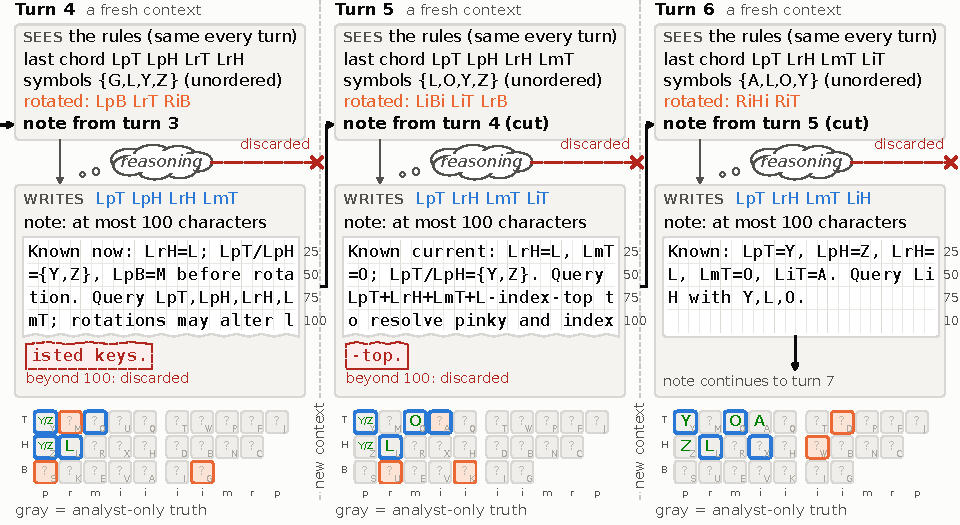
\includegraphics[width=\linewidth]{figures/relay_figA_loop.pdf}\\[5pt]
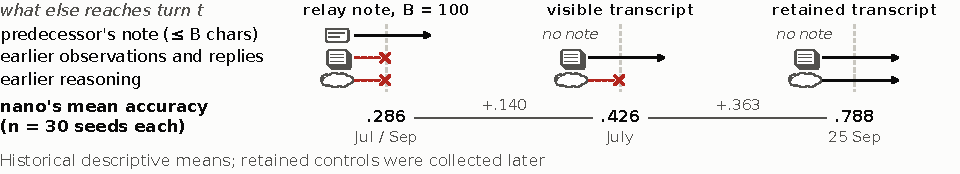
\includegraphics[width=\linewidth]{figures/relay_figA_regimes.pdf}
\caption{Inputs and notes across relay turns, with transcript controls for comparison. Top: turns 4--6 of one stored GPT-5.6 Luna episode (free-form notes, $B{=}100$ characters, seed 0). Each fresh instance receives the rules, the current observation and one note; earlier transcript and reasoning are discarded. Chords return unordered symbol sets. Key names follow the model's notation (LpT: left pinky, top row). Green shows what the note states, blue outlines the keys pressed, and orange marks keys named in the rotation notice. Small gray letters show the hidden layout as analyst annotations; the model never sees them. Cards show outgoing, not incoming, notes. Bottom: the three interfaces and GPT-5.4 Nano's historical mean board accuracy (fraction of keys correct; $n{=}30$ seeds per condition). The retained control was collected later (\Cref{tab:ladder}).}
\label{fig:loop}
\end{figure}

The conditions share game rules, reference calibrations, diagnostics, seeds and baselines. Small contexts keep episode costs to cents. Most reported cells contain $n{=}10$ seed-paired episodes; some contain 15, 20 or 30, and two Sol cells contain 5. \Cref{app:cells} gives the exact $n$ for every reported text-channel cell, separated by prompt version.

\paragraph{Contributions.}
\begin{enumerate}
\item \textbf{A relay protocol}: fresh model instances pass one authored note under a hard budget. The harness rebuilds the context each turn, replays no earlier transcript or reasoning, and stores notes verbatim.
\item \textbf{A budget-matched reference}: a sound solver uses the same channel with a truncation-aware encoder and decoder (codec). Deterministic calibrations measure what this specified policy can achieve at each budget. Both codec generations are archived (\Cref{sec:reference}).
\item \textbf{A scaffolding comparison}: paired-seed tests compare free-form notes, an imposed schema, a pinned self-designed notation specification (the constitution condition), and a harness-validated form. Visible-transcript and retained-reasoning controls provide separate comparators.
\item \textbf{Behavioral evidence}: a stored corpus of \relaystorednotes{} notes, including legacy and coaching-audit records; a note-format drift measure with a fixed-codec negative control; and a pixel channel with a separate fidelity probe. The main v2 text runs contain 15,930 notes, including 573 terminal outputs that no successor receives. Legacy and coaching-audit runs contain 1,792 and 779 notes, respectively. Four newer models from three providers test which findings extend beyond the original roster (\Cref{sec:added}).
\end{enumerate}

The base environment is public \citep{blindboarddata2026}. The per-model memory-tool screen costs about \$\relayfitcostnano--\$\relayfitcostsol{} before deployment (\Cref{sec:discussion}).
